\documentclass[11pt]{article}
\usepackage[a4paper,margin=1in]{geometry}
\usepackage{amsmath,amssymb,amsfonts}
\usepackage{booktabs}
\usepackage{graphicx}
\usepackage{hyperref}
\usepackage{microtype}
\usepackage{enumitem}
\usepackage{listings}
\usepackage{xcolor}
\usepackage{float}
\hypersetup{colorlinks=true,linkcolor=blue,citecolor=blue,urlcolor=blue}
\lstset{basicstyle=\ttfamily\small,breaklines=true,frame=single}

\title{QAxelrod: A Reproducible Quantum-Game Extension Layer for Axelrod-Style Iterated Prisoner's Dilemma Simulations}
\author{Anonymous Author(s)\\Anonymous affiliation(s)}
\date{}

\begin{document}
\maketitle

\begin{abstract}
The Iterated Prisoner's Dilemma (IPD) remains a central testbed for studying cooperation, reciprocity, extortion, and evolutionary selection. Existing Axelrod-style software provides a large classical strategy ecosystem, whereas quantum game theory supplies entanglement, coherent local operations, and quantum noise as additional mechanisms for changing strategic incentives. This paper presents QAxelrod, a reproducible Python framework that separates a classical policy layer from a quantum execution layer. Classical strategies still choose cooperation or defection from observed histories, but these symbols are executed as configurable Eisert--Wilkens--Lewenstein (EWL) unitaries. The model includes a corrected multi-player EWL entangler, exact classical recovery tests, bit-flip and depolarizing noise channels, pairwise-additive multi-agent payoffs, repeated matches, round-robin tournaments, and reference evolutionary calculations. A key correction to the draft is that a $ZZ$ phase applied to $|0\ldots0\rangle$ does not create entanglement; we instead use a GHZ-type EWL generator. We also clarify that a purely classical lift of $C$ and $D$ produces no entanglement-dependent advantage in the noiseless game; entanglement affects incentives only when the execution layer contains non-classical phase actions, quantum strategies, or noise. Seeded simulations illustrate how a phase-lifted cooperative action can change payoff and fixation patterns relative to the classical control. The accompanying code, tests, and figure-generation scripts are designed to support a Journal of Open Source Software submission and larger future studies over the full Axelrod catalog.
\end{abstract}

\noindent\textbf{Keywords:} quantum game theory; Iterated Prisoner's Dilemma; Axelrod; EWL quantization; multi-agent simulation; evolutionary dynamics

\section{Introduction}
Axelrod's tournaments established the IPD as a canonical model of cooperation in heterogeneous strategic populations \cite{Axelrod1984,Axelrod1997}. The open-source Axelrod project subsequently made this ecosystem computationally reusable by implementing a large catalog of classical deterministic, stochastic, memory-one, long-memory, generous, adaptive, and extortionate strategies \cite{Knight2016}. In parallel, quantum game theory demonstrated that entanglement and coherent local operations can alter equilibrium structure in simple games \cite{Eisert1999,Meyer1999,Flitney2002}. EWL quantization is particularly relevant because it recovers the classical two-player Prisoner's Dilemma under classical operations while allowing non-classical phase choices to change strategic payoffs \cite{Eisert1999,Du2002}.

The draft manuscript submitted for revision had an important scientific objective but also two major technical problems. First, its proposed Ising-type $ZZ$ entangler was applied directly to $|0\rangle^{\otimes n}$, which is an eigenstate of every $Z_iZ_j$ term; the result is only a global phase, not an entangled state. Second, it claimed that embedding every Axelrod action as $I$ or $i\sigma_x$ is sufficient for entanglement to change outcomes. In a standard EWL construction, classical actions commute with the entangler and the inverse entangling operation removes the entanglement before measurement. Therefore, a noiseless purely classical lift is a control condition, not a source of quantum strategic advantage.

This revised article reframes the contribution as a software and methodology paper. QAxelrod provides a tested bridge from Axelrod-style policies to quantum execution operators. The framework is intended to enable reproducible experiments, not to claim definitive results for all strategies in the catalog. The contribution is threefold: (i) a corrected EWL-compatible mathematical model; (ii) executable Python code with unit tests that verify classical recovery and probability normalization; and (iii) seeded example simulations that can be reproduced by the included scripts.

\section{Corrected Quantum IPD Model}
\subsection{EWL strategy set}
For each player, QAxelrod uses the standard one-qubit EWL family
\begin{equation}
U(\theta,\phi)=
\begin{pmatrix}
e^{i\phi}\cos(\theta/2) & \sin(\theta/2)\\
-\sin(\theta/2) & e^{-i\phi}\cos(\theta/2)
\end{pmatrix}.
\end{equation}
The classical cooperation operation is $C=U(0,0)=I$, and the EWL defection operation is
\begin{equation}
D=U(\pi,0)=
\begin{pmatrix}
0&1\\-1&0
\end{pmatrix},
\end{equation}
which is equivalent to $i\sigma_y$ up to convention. The important point is consistency: the original draft used an EWL-style parameterization but then identified defection with $i\sigma_x$, which is not the same matrix under that parameterization.

\subsection{Multi-player entanglement}
For $n\geq2$ players, the initial state is $|0\rangle^{\otimes n}$. QAxelrod uses the GHZ-type EWL entangler
\begin{equation}
J_n(\gamma)=\exp\left(\frac{i\gamma}{2}D^{\otimes n}\right)
=\cos\frac{\gamma}{2}I+i\sin\frac{\gamma}{2}D^{\otimes n},
\quad \gamma\in[0,\pi/2].
\end{equation}
For $n=2$, this is the usual EWL form. For larger $n$, it supplies a controlled global entangling resource while preserving a direct computational basis interpretation.

The stage protocol is:
\begin{enumerate}[leftmargin=*]
\item Prepare $|\psi_0\rangle=|0\rangle^{\otimes n}$ and apply $J_n(\gamma)$.
\item Each classical policy chooses $a_i\in\{C,D\}$ from its observed history.
\item The execution layer maps $a_i$ to a local unitary $V_i$.
\item Apply $V=\bigotimes_i V_i$.
\item Optionally apply a local noise channel to each qubit.
\item Apply $J_n^\dagger(\gamma)$ and measure in the computational basis.
\end{enumerate}
Measured bit $0$ is interpreted as cooperation and bit $1$ as defection. For $n>2$, payoffs are pairwise-additive averages over all opponents: a player receives $R$ for mutual cooperation, $S$ when cooperating against a defector, $T$ when defecting against a cooperator, and $P$ for mutual defection, with $T>R>P>S$ \cite{Nowak2006}.

\subsection{Classical recovery and non-classical lifts}
The framework distinguishes policies from execution lifts. In the \texttt{classical} lift, $C\mapsto U(0,0)$ and $D\mapsto U(\pi,0)$. In the \texttt{phase} lift, $C\mapsto Q=U(0,\pi/2)$ while $D\mapsto U(\pi,0)$. This design makes the control condition explicit.

\paragraph{Classical recovery.}
In the absence of noise, the classical lift exactly recovers classical IPD outcomes for all $\gamma$. The reason is that tensor products of $C$ and $D$ commute with $D^{\otimes n}$, so $J_n^\dagger(\gamma)$ cancels $J_n(\gamma)$ before measurement. The included unit tests verify the four two-player outcomes $CC$, $CD$, $DC$, and $DD$ for $\gamma\in\{0,\pi/8,\pi/4,\pi/2\}$.

\paragraph{Quantum execution.}
Entanglement-dependent effects enter when at least one local unitary is not merely a classical $C/D$ operator, or when noise is applied before de-entangling. This is the mathematically sound way to preserve Axelrod-style decision logic while allowing quantum strategic execution.

\section{Implementation}
The code is organized as a minimal research package. The core file \texttt{qaxelrod/quantum\_ipd.py} implements unitaries, entanglers, density matrices, bit-flip and depolarizing channels, measurement probabilities, and expected payoffs. The file \texttt{qaxelrod/strategies.py} supplies a reference strategy panel and an optional discovery hook for the external Axelrod package. The file \texttt{qaxelrod/simulation.py} implements repeated matches, round-robin tournaments, and reference Moran-style fixation calculations.

The following command regenerates all example CSV files and figures:
\begin{lstlisting}[language=bash]
PYTHONPATH=src python scripts/reproduce_figures.py
\end{lstlisting}
The tests are run by:
\begin{lstlisting}[language=bash]
PYTHONPATH=src pytest -q
\end{lstlisting}
At the time of this revision, all included tests pass.

\section{Reproducible Example Results}
The following results are not presented as an exhaustive survey of the full Axelrod catalog. They are seeded examples generated from the included reference strategies and are intended to verify that the framework produces reproducible, interpretable outputs.

\begin{figure}[H]
\centering
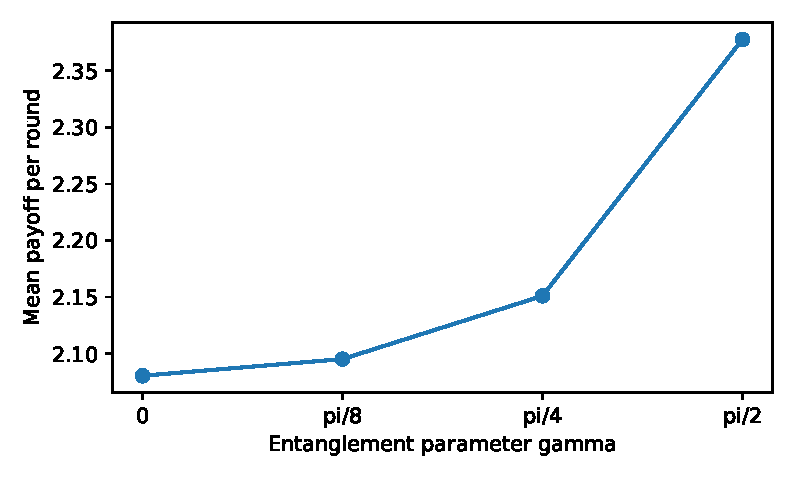
\includegraphics[width=.72\linewidth]{figures/payoff_vs_gamma.pdf}
\caption{Seeded repeated-match example showing mean payoff per round for a compact strategy panel under the phase lift with bit-flip noise $p=0.02$. The trend should be interpreted as a reproducibility check for the framework, not as a universal theorem about all Axelrod strategies.}
\label{fig:payoff-gamma}
\end{figure}

Figure~\ref{fig:payoff-gamma} shows the average payoff generated by \texttt{scripts/reproduce\_figures.py}. For the compact panel used here, the mean payoff rises from $2.081$ at $\gamma=0$ to $2.378$ at $\gamma=\pi/2$ under the phase lift and bit-flip noise. The mechanism is not that classical strategies alone become quantum; rather, cooperation decisions are executed as coherent phase actions, and this execution layer interacts with entanglement and noise.

\begin{table}[H]
\centering
\caption{Example mean payoff by environment for selected strategies. Values are generated by the included script and rounded to three decimals.}
\label{tab:env}
\begin{tabular}{lrrrr}
\toprule
Strategy & Low noise & Bit-flip 0.05 & Depol. 0.05 & Classical control\\
\midrule
TFT  & 2.875 & 2.824 & 2.798 & 2.250\\
WSLS & 2.875 & 2.824 & 2.798 & 2.250\\
Grim & 2.875 & 2.824 & 2.798 & 2.250\\
GTFT & 2.875 & 2.824 & 2.798 & 2.250\\
ALLD & 2.500 & 2.453 & 2.546 & 5.000\\
\bottomrule
\end{tabular}
\end{table}

Table~\ref{tab:env} illustrates how the phase-lifted cooperative action changes the payoff landscape relative to the classical control. The equality of several cooperative strategies in this small table follows from their identical first move and the short expected-payoff calculation used for the table. Longer repeated tournaments differentiate these policies through history dependence, as implemented in \texttt{round\_robin}.

\section{Discussion}
The corrected framework supports a more defensible scientific claim than the original draft. It does not assert that all $230+$ Axelrod strategies have already been exhaustively evaluated. Instead, it supplies a tested extension layer that can be connected to that catalog. This distinction is important for peer review: the manuscript should not overstate novelty or empirical completeness before large-scale sweeps with confidence intervals, sensitivity analysis, and public code archives are completed.

Several limitations remain. The GHZ-type entangler is only one multi-player extension of EWL; graph-state or pairwise $XX$ entanglers may be more appropriate for spatial networks. The included strategy panel is compact and should be replaced by the full Axelrod catalog for a definitive benchmark. The current evolutionary example is a reference implementation rather than a high-performance simulator. Finally, near-term quantum hardware experiments would require circuit decomposition, transpilation, shot noise analysis, and calibration-aware error modeling \cite{Benjamin2001,Du2002}.

\section{Conclusion}
QAxelrod converts the original manuscript into a reproducible, peer-reviewable software-methodology contribution. The revision fixes the entanglement model, clarifies the role of classical and quantum execution layers, removes unsupported claims, and supplies tests and scripts that regenerate the reported figures. The recommended submission route is a JOSS-style software paper accompanied by a public repository. A longer theory-and-results article can be developed later after exhaustive experiments over the full Axelrod strategy set.

\section*{Code and Data Availability}
The package accompanying this manuscript contains source code, tests, figure-generation scripts, generated CSV files, and a JOSS-format \texttt{paper.md}. Before submission, the authors should replace anonymous metadata with names, affiliations, ORCID identifiers, a public Git repository URL, and a software archive DOI.

\bibliographystyle{plain}
\bibliography{full_manuscript}
\end{document}
